\section{Evaluation}
\label{sec:eval}

In this section, we evaluate the efficacy of our various tap point search
strategies, described in Section~\ref{sec:technical}, in finding tap
points useful for introspection. Our experiments are motivated by
real-world introspection applications, and so for each experiment we
describe a typical application for the tap points found. Each experiment
was also generally performed on a variety of different operating sytems,
applications, and architectures in order to evaluate TZB's ability to
handle a diverse range of introspection targets.

For the sake of readability, we have attempted to use symbolic names for
addresses wherever possible in the following results. It is hoped that
these will be more meaningful to the reader than the raw addresses, but
we emphasize that debug information is in no way required for TZB to
work.

\subsection{URL Access}
\label{sec:eval:subsec:url}

\begin{table*}
    \centering
    \small
    \begin{tabular}{|l|l|l|}
        \hline
        Browser & Caller & PC \\
        \hline
        Deb Epiphany (arm) & \texttt{WebCore::KURL::KURL+0x30} & \texttt{WebCore::KURL::init+0x70} \\
        Deb Epiphany (amd64) & \texttt{webkit\_frame\_load\_uri+0xc3} & \texttt{WebCore::KURL::init+0x368} \\ 
        Win7 IE8 (x86) & \texttt{ieframe!CAddressEditBox::\_Execute+0xaa} & \texttt{ieframe!StringCchCopyW+0x50} \\
        Win7 Firefox (x86) & \texttt{xul!nsAutoString::nsAutoString+0x1a} & \texttt{xul!nsAString\_internal::Assign+0x1d} \\
        Win7 Chrome (x86) &  \texttt{msftedit!CTxtEdit::OnTxChar+0x105} & \texttt{msftedit!CTxtSelection::PutChar+0xb8} \\
        Win7 Opera (x86) &  \texttt{Opera.dll+0x2cf6c6} & \texttt{Opera.dll+0x142783} \\
        Haiku WebPositive (x86) & \texttt{BWebPage::LoadURL+0x3a} & \texttt{BMessage::AddString+0x26} \\
        \hline
    \end{tabular}
\caption{Tap points found that write the URL typed into the browser by
the user.}
\label{tbl:url}
\end{table*}

As with file access, monitoring visited URLs is likely to be of use to
host-based intrusion detection and prevention systems. For example, an
IDS may wish to verify that outgoing requests were initiated by a human
rather than malware on the users's machine, or match URLs visited
against a blacklist of malicious sites. This poses a challenge for
existing introspection solutions, as URL load notification is not
generally exposed by a public API, and the data resides in a user
application (the browser).

To find URL tap points, we created training executions by visiting a set
of three URLs (Google, Facebook, and Bing) the following operating
systems and browsers: Epiphany on Debian squeeze (armel and amd64);
Firefox 16.0.2, Opera 12.10, and Internet Explorer 8.0.7601.17514 on
Windows 7 SP1 (x86); and WebPositive r580 on Haiku (x86). As with the
file access case, we used the \texttt{stringsearch} plugin to search for
the ASCII and UTF-16 representations of the three URLs, and then
validated each tap point found to ensure that it wrote only the desired
data. The results can be seen in Table~\ref{tbl:url}.

\subsection{TLS/SSL Master Secrets}
\label{sec:eval:subsec:ssl}

\begin{table*}
    \centering
    \small
    \begin{tabular}{|l|l|l|l|}
        \hline
        Client & Caller & PC & Process \\
        \hline
        Deb OpenSSL (arm) & \texttt{tls1\_generate\_master\_secret+0x9c} & \texttt{tls1\_PRF+0x90} & openssl \\
        Deb OpenSSL (amd64) & \texttt{ssl3\_send\_client\_key\_exchange+0x437} & \texttt{tls1\_generate\_master\_secret+0x108} & openssl \\
        Deb Epiphany (arm) & \texttt{md\_write+0x74} & \texttt{md5\_write+0x68} & epiphany \\ 
        Deb Epiphany (amd64) & \texttt{md\_write+0x60} & \texttt{md5\_write+0x49} & epiphany \\ 
        Haiku WebPositive (x86) & \texttt{tls1\_generate\_master\_secret+0x65} & \texttt{tls1\_PRF+0x14b} & WebPositive \\
        Win7 Chrome (x86) & \texttt{chrome!NSC\_DeriveKey+0x1241} & \texttt{chrome!TLS\_PRF+0xa0} & chrome.exe \\
        Win7 IE8 (x86) & \texttt{ncrypt!Tls1ComputeMasterKey@32+0x57} & \texttt{ncrypt!PRF@40} & lsass.exe \\
        Win7 Firefox (x86) & \texttt{softokn3!NSC\_DeriveKey+0xe85} & \texttt{freebl3!TLS\_PRF+0xbb} & firefox.exe \\
        Win7 Opera (x86) & \texttt{Opera.dll+0x2eb06e} & \texttt{Opera.dll+0x50251} & opera.exe \\
        \hline
    \end{tabular}
\caption{Tap points found that write the SSL/TLS master secret for each
SSL/TLS connection. These keys can be used to perform transparent
interception of SSL traffic without man-in-the-middle.}
\label{tbl:ssl}
\end{table*}

Monitoring SSL/TLS-encrypted traffic is a classic problem for intrusion
detection systems. Currently, hypervisor- or network- based IDSes that
wish to analyze encrypted traffic must perform a man-in-the-middle
attack on the connection, presenting a false server certificate to the
client. Not only does this require the client to cooperate by trusting
certificates signed by the intrusion detection system, it also takes
control of the certificate verification process out of the hands of the
client---a dangerous step, given that many existing SSL/TLS interception
proxies have a history of certificate trust
vulnerabilities~\cite{JarmocBHEU2012}.

Instead of a man-in-the-middle attack, we can instead use TZB to find a
tap point that reads or writes the SSL/TLS master secret for each
encrypted connection. Because this secret must be generated for each
SSL/TLS connection, if we can find such a tap point, it can then be
provided to the IDS to decrypt and, if necessary, modify the content of
the SSL stream.

To find the location of these tap points, we a modified copy of
OpenSSL's \texttt{s\_server} utility that prints out the SSL/TLS master
key any time a connection is made. We then recorded executions in which
we visited the server with each of our tested SSL clients, and noted the
SSL/TLS master secret. Finally, we used \texttt{stringsearch} to search
for a tap point that wrote the master key, and verified that the tap
wrote exactly one master key per connection. For this test, we used:
OpenSSL s\_client 0.9.8 on Debian squeeze (armel), OpenSSL s\_client
0.9.8 and Epiphany 2.30.6 on Debian squeeze (amd64), and Firefox
16.0.2, Google Chrome 23.0.1271.64, Opera 12.10, and Internet Explorer
8.0.7601.17514 on Windows 7 SP1 (x86). The results are shown in
Table~\ref{tbl:ssl}.

There is one particular point of interest to observe in these results.
In the case of Epiphany on Debian, we found that one level of callstack
information was \emph{not} sufficient, in contrast to the other results
reported here---with only the immediate caller, the tap point contains
more data than just the SSL/TLS master secret. This is because the
version of Epiphany uses SSLv3 to make connections, and the
pseudo-random function (PRF) used in SSLv3 has the form
\[ MD5(SHA1(\ldots))\] The other implementations instead use TLSv1.0,
where the PRF has the form \[ MD5(\ldots) \oplus SHA1(\ldots) \] This final
XOR operation is done from a unique program point, so the tap point that
results from it contains only TLS master keys. This points to a
potential downside of using tap points for introspection: it is not
always clear in advance how many levels of call stack information will
be required.

We were successful in locating tap points for all SSL/TLS clients tested.
We note that uncovering similar information using traditional techniques
would have required significant expertise and reverse engineering of
both open source and proprietary software.

\subsection{SSL Malware}
\label{sec:eval:subsec:sslmal}

The need to snoop on SSL-encrypted connections arises in malware
analysis as well. Two features distinguish this case from that of
intercepting the traffic of benign SSL clients presented in the previous
section. First, the ability to decrypt the traffic without a man in the
middle is even more important: in contrast to benign clients, we cannot
assume that malware will accept certificates signed by our certificate
authority. Second, we cannot rely on having access to the server's
master secret, as the server is under the attacker's control. This means
that our previous strategy of using a simple string search for the
master secret will not work here.

Instead, we located the tap point in the SSL-enabled malware by creating
a PANDA plugin called \texttt{keyfind} that performs trial decryption on
a packet sent by the malware using each possible 48-byte sequence
written to memory as a key.  Although this is much slower than a string
match, it is the only available option, since the key is not known in
advance.

To test the plugin, we obtained a copy of a version of the Sykipot
trojan released around October 31st, 2012~\cite{sandymal} (MD5:
\texttt{34a1010846c0502f490f17b66fb05a12}). We then created a recording
in which we executed the malware; simultaneously, we captured network
traffic using \texttt{tcpdump}. We noted that the malware made several
encrypted connections to \url{https://www.hi-techsolutions.org/}, and
provided one of the encrypted packets from these connections as input to
the \texttt{keyfind} plugin. The plugin found the same tap point as the
Windows 7 IE8 experiment described in the previous section, indicating
that both the malware and IE8 likely use the same underlying system
mechanism to make SSL connections. The key found was able to decrypt the
connections contained in the packet dump.\footnote{The malware also has
a second layer of encryption, which custom and not based on SSL; we did
not attempt to decrypt this second layer.}

\subsection{File Access}
\label{sec:eval:subsec:file}

\begin{table*}
    \centering
    \small
    \begin{tabular}{|l|l|l|}
        \hline
        Target & Caller & PC \\
        \hline
        Debian (amd64) & \texttt{getname+0x13e} & \texttt{strncpy\_from\_user+0x52} \\ 
        Debian (arm) & \texttt{getname+0x88} & \texttt{\_\_strncpy\_from\_user+0x10} \\
        Haiku (x86) & \texttt{EntryCache::Lookup+0x27} & \texttt{hash\_hash\_string+0x1b} \\
        FreeBSD (x86) & \texttt{namei+0xd1} & \texttt{copyinstr+0x38} \\
        Windows 7 (x86) & \texttt{ObpCaptureObjectName+0xcb} & \texttt{memcpy+0x33} \\
        \hline
    \end{tabular}
\caption{Tap points found for file access on different operating systems.}
\label{tbl:file}
\end{table*}

Monitoring file accesses is a requirement for many host-based security
applications, including on-access anti-virus scanners. Thus, locating a
tap point at which systemwide file accesses can be observed is of
considerable importance. However, because previous approaches to the
introspection problem~\cite{Dolan-Gavitt:2011uq,Fu:2012fk} passively
retrieve information from the guest and are not event-driven, they
cannot be used in this scenario.

To find such a tap point, we created recordings in which we opened files
in various operating systems. Specifically, in each OS we created 100
files, each named after ten successive digits of $\pi$. The operating
systems chosen for this test were: Debian squeeze (amd64), Debian
squeeze (armel), Windows 7 SP1 32-bit, FreeBSD 9.0, and Haiku R1 Alpha
3 (all on x86). We then searched for tap points that wrote strings
matching the ASCII and UTF-16 encodings of the filenames using the
\texttt{stringsearch} analysis plugin. The UTF-16 encodings were
included because it was known that Windows 7 uses UTF-16 for strings
pervasively, allowing us to surmise that filenames would likely be
UTF-16 encoded. Finally, we looked at the tap points found by
\texttt{stringsearch}, and validated them by hand.

The results are shown in Table~\ref{tbl:file}. For most of the operating
systems we had no difficulty finding a tap point that contained the name
of each file as it was accessed. The one exception was Windows 7, where
the most promising tap point not only wrote file results, but also a
number of unrelated objects such as registry key names. As in the SSL
case, the root cause of this was insufficient calling context: in
Windows several different things fall under the umbrella of a ``named
object'', and these were all being captured at this tap point. We found
that four levels of calling context were sufficient to restrict the tap
point to just file accesses; the ``deepest'' caller was
\texttt{IopCreateFile} (which, despite its name, is used for both
opening existing files and creating new ones).

\subsection{Finding \large \texttt{dmesg}}
\label{sec:eval:subsec:dmesg}

\begin{table*}
    \centering
    \small
    \begin{tabular}{|l|l|l|l|l|}
        \hline
        OS & Caller & PC & Kernel? & Rank \\
        \hline
        FreeBSD (x86) & \texttt{msglogstr+0x28} & \texttt{msgbuf\_addstr+0x19a} & Yes & 1 \\
        Haiku (x86) & \texttt{ring\_buffer\_peek+0x59} & \texttt{memcpy\_generic+0x14} & Yes & 1 \\
        Debian (arm) & N/A & \texttt{do\_syslog+0x18c} & Yes & 4 \\
        Debian (amd64) & N/A & \texttt{do\_syslog+0x163} & Yes & 4 \\ 
        Minix (x86) & \texttt{0x190005ee} & \texttt{0x190009d4} & No & 8 \\
        \hline
    \end{tabular}
\caption{Tap points that write the system log (\texttt{dmesg}) on
several UNIX-like operating systems. All tap points were located in the
kernel, except for Minix, which is a microkernel.}
\label{tbl:dmesg}
\end{table*}

System logs are an invaluable resource, both for security and system
administration. In an introspection-based security system, for example,
one might want to find a tap point that contains the system's logs so
that they can be stored securely outside the guest virtual machine.
However, because the format of system logs is particular to each OS, we
need some mechanism that can find tap points that write data that
``looks like'' a log based on an exemplar. The statistical search
described in Section~\ref{sec:technical:subsec:knownunk} is a good fit
for this task: by training on the output of \texttt{dmesg} on one
OS, we can find \texttt{dmesg}-like tap points on other systems.

To locate these system log tap points, we first created a training
exemplar by running the \texttt{dmesg} command on a Debian sid (amd64)
host, and computing the bigram probabilities for the output. We then
created recordings in which we booted five operating systems: Debian
squeeze (armel), Debian squeeze (amd64), Minix R3-2.0 (i386), FreeBSD
9.0-RELEASE (i386), and Haiku R1 Alpha 3 (i386), and computed the same
bigram statistics. We then sorted the tap points seen in each operating
system boot according to their Jensen-Shannon distance from the training
distribution, and manually examined data written by the tap point for
each of the top 30 results in each operating system. Table~\ref{tbl:dmesg}
shows, for each operating system tested, the tap point that we determined to be
the system log, and its rank in the search results.

We can see that in all cases the correct result is in the top 10. There
are two additional features about Table~\ref{tbl:dmesg} that bear
mentioning. First, the reader will note that the two Debian systems have
a caller of ``N/A''. This is because the memory writes that make up
\texttt{dmesg} are done in \texttt{do\_syslog}, which is called from
multiple functions. In these cases, including the caller splits up
information that is semantically the same. We detected this case by
noticing that several of the top-ranked results in the Linux experiments
had the same program counter, and that they appeared to contain
different sections of the same log. Second, the tap point found for
Haiku was also incomplete---some lines were truncated. By using our tap
point correlation plugin, we determined that we were missing a second
tap point that was correlated with the main one; the two together formed
the write portions of a \texttt{memcpy} of the log messages. Once this
second tap point was included, we could see all the log messages
produced by Haiku.

We also attempted to find an analogous log message tap point on Windows
7, but were not successful. This is a result of the way Windows logging
works: rather than logging string-based messages, applications and
system services create a manifest declaring possible log events, and
then refer to them by a generated numeric code. Human-readable messages
are not stored, and instead are generated when the user views the log.
This means that there is no tap point that will contain log messages of
the type used in our \texttt{dmesg} training, and the methods described
in this paper are largely inapplicable unless a training example for the
binary format can be found. However, because there event log query API
is public~\cite{evtquery}, existing tools such as
Virtuoso~\cite{Dolan-Gavitt:2011uq} might be a better fit for this use
case.

Anecdotally, the ability to uncover a tap point that writes the kernel
logs has also been useful for diagnosing problems when adding support
for new platforms to QEMU. For an unrelated research task, we attempted
to boot the Raspberry Pi~\cite{raspberrypi} kernel inside QEMU, but
found that it hung without displaying any output early on in the boot
process. By locating the \texttt{dmesg} tap point, we discovered that
the last log message printed was ``Calibrating delay loop...''; based on
this we determined that the guest was hung waiting for a timer interrupt
that was not yet implemented in QEMU.

\subsection{Clustering}
\label{sec:eval:subsec:cluster}

To test the effectiveness of clustering tap points based on bigram
statistics and Jensen-Shannon distance, we carried out an experiment
that compared the clusters generated algorithmically to a set of labels
generated by two of the co-authors manually examining the data. We
created six recordings representing different workloads on two operating
systems (Windows 7 and FreeBSD 9.0). From FreeBSD, we took recordings of
boot, shutdown, running applications (\texttt{ps}, \texttt{cat},
\texttt{ls}, \texttt{top}, and \texttt{vi}), and a one-minute recording
of the system sitting idle, for a total of four recordings. On Windows
we created two recordings: running applications (\texttt{cmd.exe},
\texttt{dir}, the Task Manager, Notepad), and one minute of the system
sitting idle.\footnote{Although we would have preferred to include
Windows boot and shutdown recordings, at the time our replay system had
a bug (now fixed) that prevented these recordings from being replayed.}
Table~\ref{tbl:clusttaps} shows the number of tap points found in each
of the recordings; we can see that the FreeBSD system is overall much
less active than the Windows 7 system during the time periods we
recorded.

Next, we sampled a subset of the tap points found in each recording.
Given that the vast majority of tap points do not write interesting
information, we opted not to sample uniformly from the all tap points
found. Instead, we performed an initial $k$-means clustering with $k =
100$, and then picked out tap points at various distances from each
cluster center. For each cluster, we chose the tap point at $\sigma$
standard deviations from the center, for $\sigma \in \left\{0, 0.5,
0.75, 1.0, 1.25, 1.5, 1.75, 2.0 \right\}$ for a total of 2,926
samples\footnote{The alert reader will note that this is smaller than
the 4,800 samples one would expect from taking 8 samples from 100
clusters in each of 6 recordings. This is because some clusters did not
have very high variance, and so in many cases there were fewer than 8
samples at the required distance from the center.}. Finally, we dumped
the data from each of the sampled tap points, blinded them by assigning
each a unique id, and then provided the data files to our two labelers.
Each labeler independently assigned labels to each of the samples using
the labels described in Table~\ref{tbl:clustlabels}, and the two
labelers then worked together to reconcile their labels.

Finally, we ran a $k$-means clustering with $k = 10$; $10$ was chosen
because it was a round number reasonably close the number of labels our
human evaluators gave to the data. We then used the Adjusted Rand
Index~\cite{Hubert:1985zr} to score the quality of our clustering
relative to our hand-labeled examples. The Adjusted Rand Index for a
clustering ranges from -1 to 1; clusterings which are independent of the
hand labeling will receive a score that is negative or close to zero. As
can be seen in Table~\ref{tbl:clustqual}, our clustering was generally
of poor quality and did not match up very well on the hand-labeled
samples.

Based on these results, we conclude that at present, clustering does not
appear to work very well for our purposes. There is some hope, however.
In an effort to understand why our clustering performed so poorly, we
created a confusion matrix for the Win7 Apps recording, which can be
seen in Figure~\ref{fig:win7apps}. The values along the diagonal
represent the fraction of taps that were correctly assigned to the
same cluster when a human had assigned them to the same cluster. The
remaining cells represent the fraction of taps correctly assigned to
different clusters when a human had assigned them different labels. The
magenta cells indicate that we did not have enough examples to make a
comparison. In short: light cells mean the clustering performed well on
that pair of labels, dark cells mean it performed poorly. From this we
can see that for many of the labels of human interest (i.e., those which
are primarily text-based) the clustering performed reasonably well,
but it performed poorly on tap points that contained binary data. This
helps explain its poor overall performance, since the vast
majority---90.8\%---of the samples in our labeling were not text-based.
In future work we hope to carry out further experiments to determine
whether the clusters found are useful in reducing the amount of data a
human reverse engineer would have to look through.

\begin{figure}
    \centering
    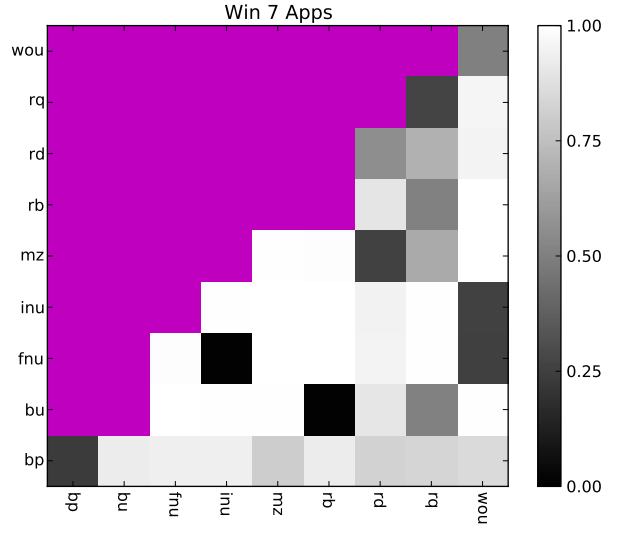
\includegraphics[width=3in]{figures/win7apps.png}
    \caption{Confusion matrix for our clustering of the Windows 7 Apps
    recording compared to handmade labels. Lighter cells indicate that
    the clustering matched the hand-labeled samples well for that
    pair of labels.}
    \label{fig:win7apps}
\end{figure}

\begin{table}
    \centering
    \small
    \begin{tabular}{|l|l|r|}
        \hline
        Abbrv. & Description & Count \\
        \hline
        bp  &  binary pattern &  2318  \\
        rd  &  repeated dword &  400  \\
        mz  &  mostly zero &  141  \\
        rq  &  repeated quadword &  19  \\
        fnu  &  filenames unicode &  8  \\
        woa  &  words ascii &  8  \\
        wou  &  words unicode &  7  \\
        inu  &  integers unicode &  6  \\
        bu  &  binary uniform &  5  \\
        ura  &  URLs ascii &  5  \\
        rs  &  repeated short &  4  \\
        fna  &  filenames ascii &  2  \\
        rb  &  repeated byte &  2  \\
        vr  &  very redundant &  1  \\
        \hline
    \end{tabular}
\caption{Labels given to the sampled tap points by human evaluators,
along with the number of times each occurred.}
\label{tbl:clustlabels}
\end{table}

\begin{table}
    \centering
    \small
    \begin{tabular}{|l|r|}
        \hline
        Recording & Tap Points \\
        \hline
        Win7 Apps        & 1293429 \\
        Win7 Idle        & 520032 \\
        FreeBSD Boot     & 507900 \\
        FreeBSD Shutdown & 152899 \\
        FreeBSD Apps     & 60573 \\
        FreeBSD Idle     & 15569 \\
        \hline
    \end{tabular}
\caption{Number of tap points in each recording.}
\label{tbl:clusttaps}
\end{table}

\begin{table}
    \centering
    \small
    \begin{tabular}{|l|r|}
        \hline
        Recording & ARI \\
        \hline
        FreeBSD Apps & 0.018 \\
        FreeBSD Boot & 0.048 \\
        FreeBSD Idle & 0.021 \\
        FreeBSD Shutdown & 0.074 \\
        Win7 Apps & 0.029 \\
        Win7 Idle & -0.003 \\
        \hline
    \end{tabular}
\caption{Quality of clustering as measured by the Adjusted Rand Index,
which ranges from -1 to 1, with 1 being a clustering that perfectly
matches the hand-labeled examples.}
\label{tbl:clustqual}
\end{table}
